\documentclass[12pt]{article}

% set margins and spacing
\addtolength{\textwidth}{1.3in}
\addtolength{\oddsidemargin}{-.65in} %left margin
\addtolength{\evensidemargin}{-.65in}
\setlength{\textheight}{9in}
\setlength{\topmargin}{-.5in}
\setlength{\headheight}{0.0in}
\setlength{\footskip}{.375in}
\renewcommand{\baselinestretch}{1.0}
\linespread{1.0}

% load miscellaneo`us packages
\usepackage{csquotes}
\usepackage[american]{babel}
\usepackage[usenames,dvipsnames]{color}
\usepackage{graphicx,amsbsy,amssymb, amsmath, amsthm, MnSymbol,bbding,times, verbatim,bm,pifont,pdfsync,setspace,natbib}

% enable hyperlinks and table of contents
\usepackage[pdftex,
bookmarks=true,
bookmarksnumbered=false,
pdfview=fitH,
bookmarksopen=true,hyperfootnotes=false]{hyperref}

% define environments
\newtheorem{definition}{Definition}
\newtheorem{fact}{Fact}
\newtheorem{result}{Result}
\newtheorem{proposition}{Proposition}



\begin{document}
\title{Development: The link between Manufacturing Employment and GDP in Developed and Developing Countries}
\author{Filippo Donà\thanks{Syracuse University, Economics Department. Email: kbuzard@syr.edu.} \and Lucia Rios-Luy\thanks{abc} \and Meghavarshini Iska \thanks{Syracuse University, Economics Student. Email: Meiska@syr.edu}}
\date{\vskip-.1in \today}
\maketitle

\vskip.3in
\begin{center} {\bf Abstract} \end{center}

\begin{quote}
{\small We examine the link between GDP growth and manufacturing employment, hypothesizing that there is a negative relationship between manufacturing employment and GDP; As manufacturing employment decreases, GDP increases. We source statistics
from Our World in Data charts, which examine these variables in all countries around the globe.
We create a distinction between developing and developed countries, setting the threshold at USD 20.000 Annual GDP per capita. We conduct a correlation test to compare these variables across both economies. 
The research conducted supports the hypothesis that manufacturing plays a more significant role in driving economic growth in developing countries compared to developed ones. The positive correlation in developing countries underscores the critical role of industrialization in early stages of economic
growth. In contrast, the negative correlation in developed countries highlights the global transition.}
\end{quote}

\bigskip

\section{Introduction} \label{sec:introduction}

Answer the questions
\begin{enumerate}
    \item \textbf{Why should the reader care? / Why is the topic important?} (required)
    \item Why did you choose this topic? (optional)
    \item \textbf{What question will you answer? How will you do it?} (required)
        \begin{enumerate}
            \item If your theory/hypothesis fit in one paragraph, include it here. If it is longer, make it a separate section after the lit review. EITHER OPTION IS FINE as long as the length is sufficient/appropriate for your project.
        \end{enumerate}
    \item \textbf{What did you find?} (required)
    \item \textbf{Give a "road map" of the paper. Where will the reader find the various parts of your work?} (required)
\end{enumerate}

\section{Literature Review} \label{sec:literature}


% Discuss at least five papers that are closely related to your results (more is better). Explain how they're related. Did you find something similar, or different? Did you look at a different context? Different time period? Different level of detail?

Industrialization continues to be a critical driver of economic growth and development, but manufacturing has increasingly become concentrated in some countries. The Industrial Revolution, which began in Britain around the late 18th century, catalyzed this economic shift, with nations like Britain leading in technological advancements and rising per capita incomes by the early 19th century (Allen, 2009). However, in the 21st century, manufacturing sectors have become concentrated in specific regions, with developing nations like those in Africa and parts of Asia still struggling to catch up (Rodrik, 2016). Despite these disparities, the overall significance of industrialization has not diminished, but its unequal distribution continues to contribute to income gaps that emerged as early as the mid-19th century (Pomeranz, 2000).

\section{Theoretical Analysis}
\label{sec:theory}
%Optional–may include in intro if it’s short.
This paper examines how manufacturing employment has affected growth development over time and place. Explicitly, we look at how the manufacturing employment sector will impact the gross domestic product per capita (GDP per capita) in developed and developing countries. Within our data analysis, we have observed that the correlation is different in developed and developing countries. In contrast, in developed countries, we can see a negative and positive correlation within developing countries. As manufacturing employment decreases, GDP increases in developed regions, and as manufacturing employment increases, so does GDP per capita in developing countries. This idea stems from the economic transformation seen in advanced nations, where progress in technology and the rise of service-based industries have reduced reliance on manufacturing labor yet continued to fuel GDP expansion. Using automation and innovation, developed economies achieve greater productivity with a smaller manufacturing workforce. In contrast, developing nations with lower GDP per capita base their growth on using natural resources and a heavy dependence on agricultural growth. In addition, they have a great potential for manufacturing employment, as they have a high low-wage labor market. This theoretical perspective forms the basis for our empirical investigation into the relationship between manufacturing employment and economic growth in different stages of development.


\section{Data}
\label{sec:data}


The Our World in Data chart data gives us an overview of the different world indicators that estimate the position of each country's economy and development projection. The Data chart dataset has been sourced from international organizations, national statistical agencies, and multiple surveys that cover social, economic, and environmental indicators for nearly all countries from 1990 to the present day Each data point is supposed to help show how manufacturing employment and GDP have changed over the years using indicators for each country. We sectioned two variables, ``Manufacturing jobs as a share of total employment'' and ``GDP per Capita,'' into developing and developed to observe the effects of manufacturing employment on developing and developed countries' growth rates.

The Our World in Data set includes over a hundred variables, but we solely focus on GDP per capita and Manufacturing jobs as a share of total employment, which offer a detailed insight into development trends on a global scale. The data provided in this data is crucial for policymakers as it offers critical insights and long-term patterns for development across different regions of the world.

For our purposes, we have taken that any country with a GDP per Capita equal to or greater than 20,000 USD will be considered a developed country and below as developing. 


The data set is integral, for us to tabulate certain variables to form initial descriptive links. We are working with variables, such as GDP, and manufacturing employment within the data set. In a comparative analysis, we would use "codebook" to establish how often a variable is present in a dataset, and also to be able to derive and analyze the mean, median, and standard variation.

\subsection{Descriptive Statistics}

\textbf{In developing countries:}
\begin{itemize}
\item \textbf{Manufacturing employment share:} Mean of 10.55 percent, with a standard deviation of 4.88 percent. This indicates relatively low levels of industrialization and significant variability among countries.
\item \textbf{GDP per capita:} Mean of 17,957.71 USD, with a standard deviation of 20,173.73 USD. This reflects both economic disparity and uneven development across regions.
\end{itemize}

\textbf{In developed countries:}
\begin{itemize}
\item \textbf{Manufacturing employment share:} Mean of 14.38 percent and a standard deviation of 5.88 percent, reflecting more advanced industrial structures with moderate variation.
\item \textbf{GDP per capita:} Mean of 36,008.51 USD, with a standard deviation of 21,577.48 USD, indicating greater economic stability and higher income levels.
\end{itemize}



\section{Results}
\label{sec:result}

The analysis evaluated the relationship between manufacturing employment and GDP per capita across developed and developing countries from 1990 to 2019.As manufacturing employment decreases, GDP increases, which indicates a negative relationship between manufacturing employment and GDP. The null hypothesis that goes along with our hypothesis is that there is no relationship between manufacturing employment and GDP. Descriptive statistics revealed distinct patterns between these two groups, reflecting their varying stages of industrialization and economic growth.

\subsection{Graphical Trends}


\begin{itemize}
\item \textbf{Developing countries:} 
\begin{figure}
    \centering
    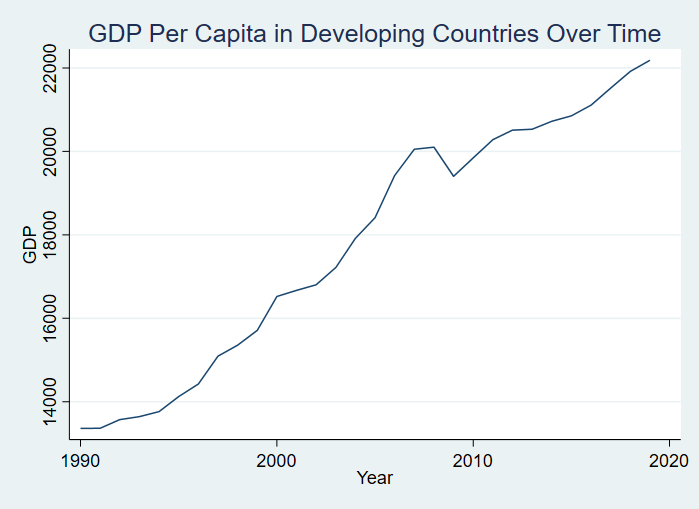
\includegraphics[width=0.5\linewidth]{GDP DEVELOPING GRAPH.png}
    \caption{Enter Caption}
    \label{fig:enter-label}
\end{figure}
\begin{figure}
    \centering
    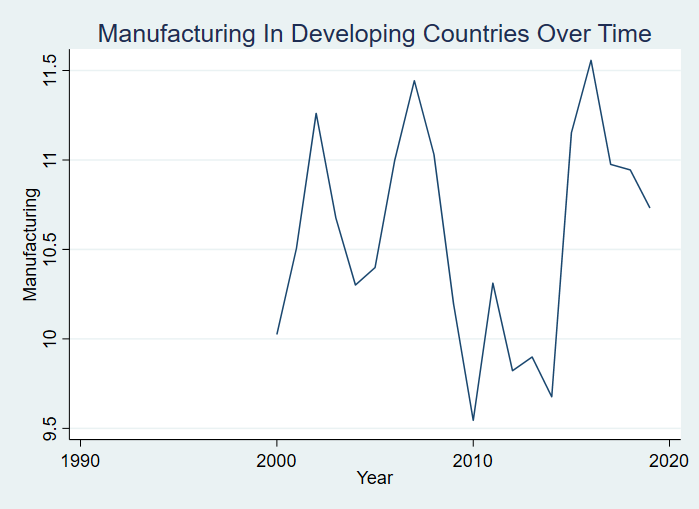
\includegraphics[width=0.5\linewidth]{FINAL GRAPH MFT DEVELOPING.png}
    \caption{Enter Caption}
    \label{fig:enter-label}
\end{figure}
\item Manufacturing employment shares exhibited fluctuations but generally declined after 2010. However, GDP per capita followed a steady upward trajectory, suggesting that factors beyond manufacturing, such as technological adoption or service sector expansion, are driving economic growth.

\item \textbf{Developed countries:} 
\begin{figure}
    \centering
    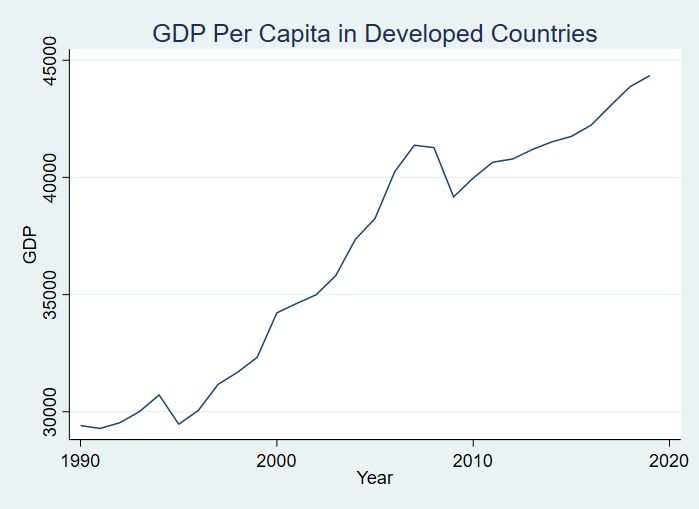
\includegraphics[width=0.5\linewidth]{FINAL FINAL GDP DEVELOPED.png}
    \caption{Enter Caption}
    \label{fig:enter-label}
\end{figure}
\begin{figure}
    \centering
    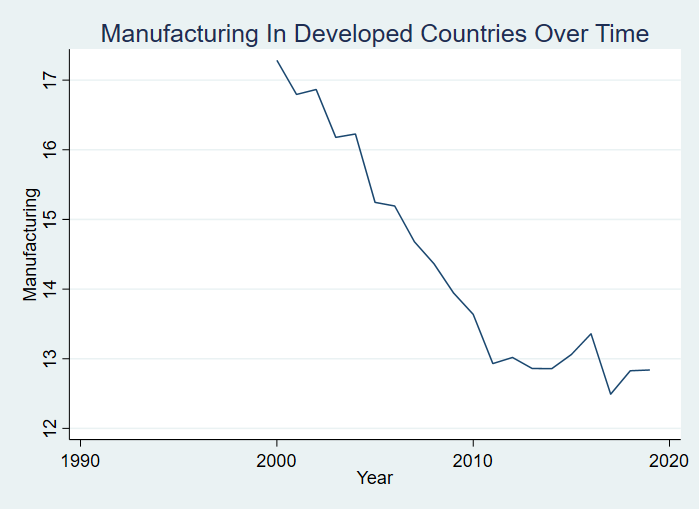
\includegraphics[width=0.5\linewidth]{FINAL FINAL MANU DEVELOPED.png}
    \caption{Enter Caption}
    \label{fig:enter-label}
\end{figure}

\item Manufacturing employment shares consistently declined over the study period, reflecting ongoing de-industrialization. Despite this, GDP per capita showed steady growth, highlighting the role of advanced industries, automation, and high-productivity sectors in sustaining economic progress.
\end{itemize}

\subsection{Correlation Analysis}
A correlation test will be conducted to compare developing to developed countries and economies, and we will graph our two main variables, GDP and manufacturing employment.
\begin{itemize}
\item \textbf{Developing Countries:} The correlation between manufacturing employment share and GDP per capita was \textbf{0.2710}, with a p-value of 0.0000, indicating a positive relationship. This suggests that higher manufacturing employment shares are associated with higher GDP per capita, reinforcing the importance of industrialization in early stages of economic development.
\item \textbf{Developed Countries:} The correlation between manufacturing employment share and GDP per capita was \textbf{-0.3601}, with a p-value of 0.0000, indicating a statistically significant negative relationship. This reflects the shift toward service-oriented economies in developed nations, where GDP growth continues despite declining manufacturing employment.
\end{itemize}


\subsection{Interpretation of Results}

These findings support the hypothesis that manufacturing plays a more significant role in driving economic growth in developing countries compared to developed ones. The positive correlation in developing countries underscores the critical role of industrialization in early stages of economic growth. In contrast, the negative correlation in developed countries highlights the global transition toward service-oriented economies.

This analysis also reveals the uneven benefits of industrialization across regions. Developing countries can leverage industrialization to reduce economic disparity, while developed countries must focus on diversifying their economies and embracing innovation to sustain growth.

\subsection{Limitations}

This study’s reliance on aggregate data may mask important variations between individual countries. Additionally, gaps in data reporting, especially in developing countries, could affect the validity of the results. Future research could incorporate more specific data and explore the effects of other sectors, such as technology and services, on GDP growth

\section{Discussion}
\label{sec:discussion}


The analysis relies on aggregate data, which may mask important variations between countries. Further, many developing countries lack continuous data, with some years not reporting any numbers, causing sudden fluctuations in manufacturing data and its visual representation. On a similar note, the time frame for developed economies (2000–2019) and developing economies (1990–2019) varies, potentially affecting the consistency of the analysis.
In developed countries, the progressive switch to tertiary industries plays a significant role in GDP changes, as demonstrated by a relatively low R-squared.

Further research should monitor future changes, directly seeking out data from respective government and independent sources, and filling in blanks.


\section{Conclusion}
\label{sec:conclusion}

Manufacturing and economic growth are unequivocally linked. Previous literature has largely focused on the shift toward manufacturing across time, starting from the industrial revolution, and the income gaps that have risen across the world today.  We examined the relationship between manufacturing and GDP, and how this differs between developed and developing countries.

\newpage
\section*{Bibliography}
\singlespacing
\setlength\bibsep{0pt}

You can either explicitly include your list of references, or you can learn to use BibTex so that it includes the references automatically.

Either way, this list should include ONLY the papers (reports, book chatpers, etc.) that you actually cite in the text (no extra).

At the same time EVERYTHING you cite in the main text must have an entry here (no references in text that don't have something here).

You can choose which citation style to follow. Whichever you choose, you must follow it consistently.

\newpage
\section*{Data Appendix} \label{sec:appendixa}
\addcontentsline{toc}{section}{Appendix A}

Once the data is categorized, we manually selected all countries, then click on the download, clicking on the "Data" option before downloading the data set completely. 

\end{document}
